\documentclass[12pt]{article}
\usepackage{amsmath}
\usepackage{graphicx}
\usepackage{hyperref}
\usepackage[utf8]{inputenc}
\usepackage[spanish]{babel}
\usepackage[margin=3cm]{geometry}
\usepackage{amsfonts}
\usepackage{listings}
\usepackage[T1]{fontenc}
\usepackage{float}
\usepackage{subfig}

\title{Practica 5 - Visión por Computador.}
\author{Néstor Rodríguez Vico. DNI: 75573052C - \href{mailto:nrv23@correo.ugr.es}{nrv23@correo.ugr.es}}
\date{\today}


\lstdefinestyle{bash_style}{
	language=bash,
	frame=single,
	xleftmargin=.25in,
	upquote = true,
	basicstyle=\scriptsize,
	breakatwhitespace=false,         
	breaklines=true,                 
	captionpos=b,                    
	keepspaces=true,                 
	numbers=left,                    
	numbersep=5pt,                  
	showspaces=false,                
	showstringspaces=false,
	showtabs=false,                  
	tabsize=2
}

\lstset{style=bash_style}

\begin{document}
\maketitle

\setlength{\belowdisplayskip}{5pt} 
\setlength{\belowdisplayshortskip}{5pt}
\setlength{\abovedisplayskip}{5pt} 
\setlength{\abovedisplayshortskip}{5pt}

\section{Fourier.}

A continuación se muestra el resultado de la transformada de Fourier. Podemos ver que hay tres grupos de 4 imágenes. En el primero se muestra el resultado de aplicar la transformada a un círculo en la posición \textit{320, 320} de la imagen (el centro de la misma) y de radio \textit{5}. En el segundo grupo se muestra el resultado de aplicar la transformada a un círculo en la posición \textit{0, 0} de la imagen (esquina superior izquierda de la misma) y de radio \textit{15}. Finalmente, en el tercer grupo se muestra el resultado de aplicar la transformada a un círculo en la posición \textit{100, 190} de la imagen y de radio \textit{20}. \\

\begin{table}[H]
	\begin{tabular}{ccc}
		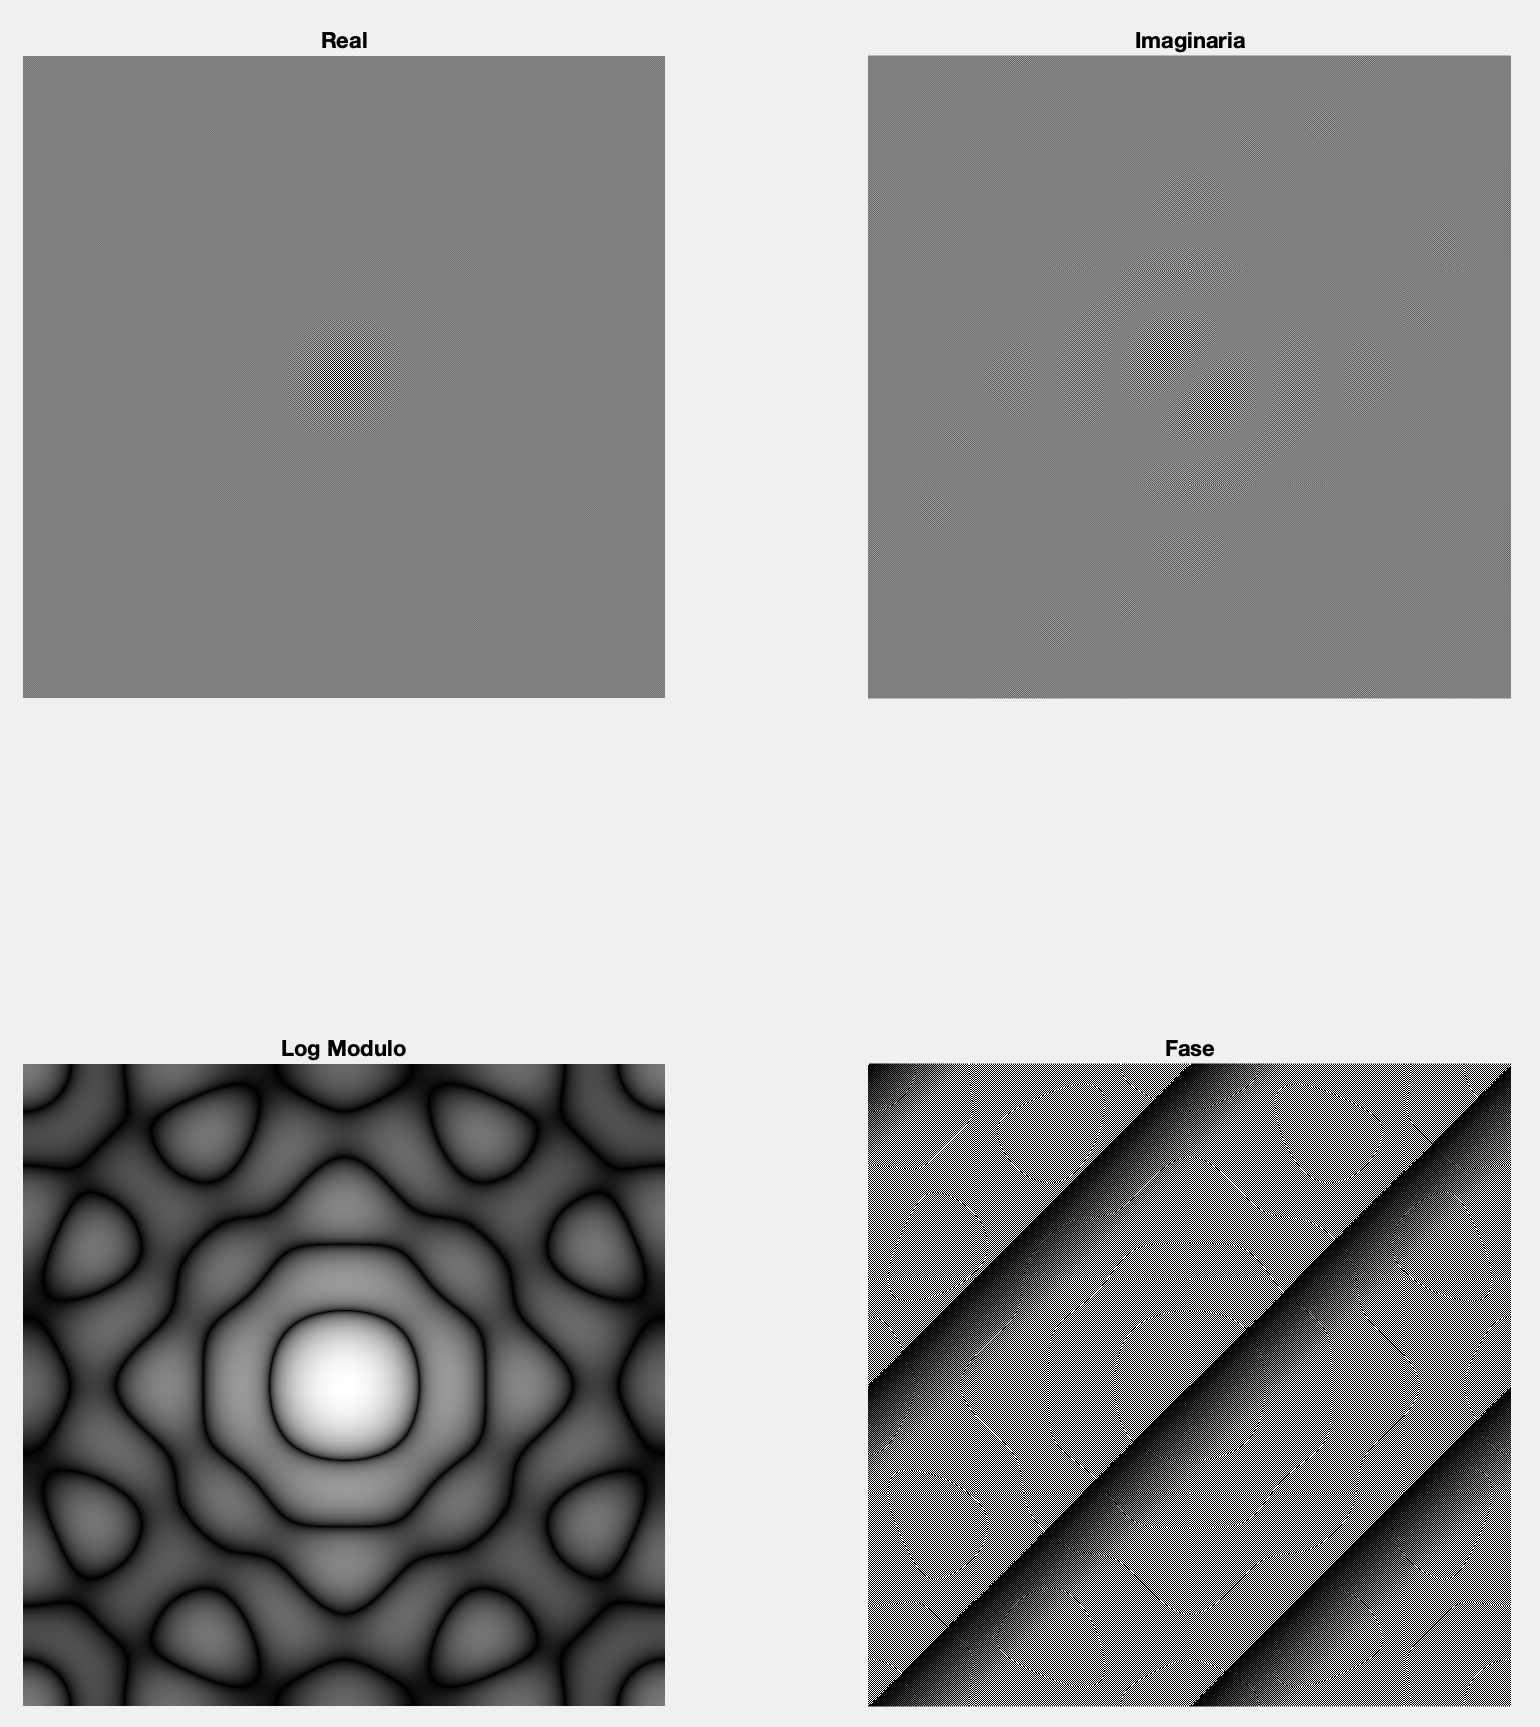
\includegraphics[width=0.3\linewidth]{images/f1.png} & 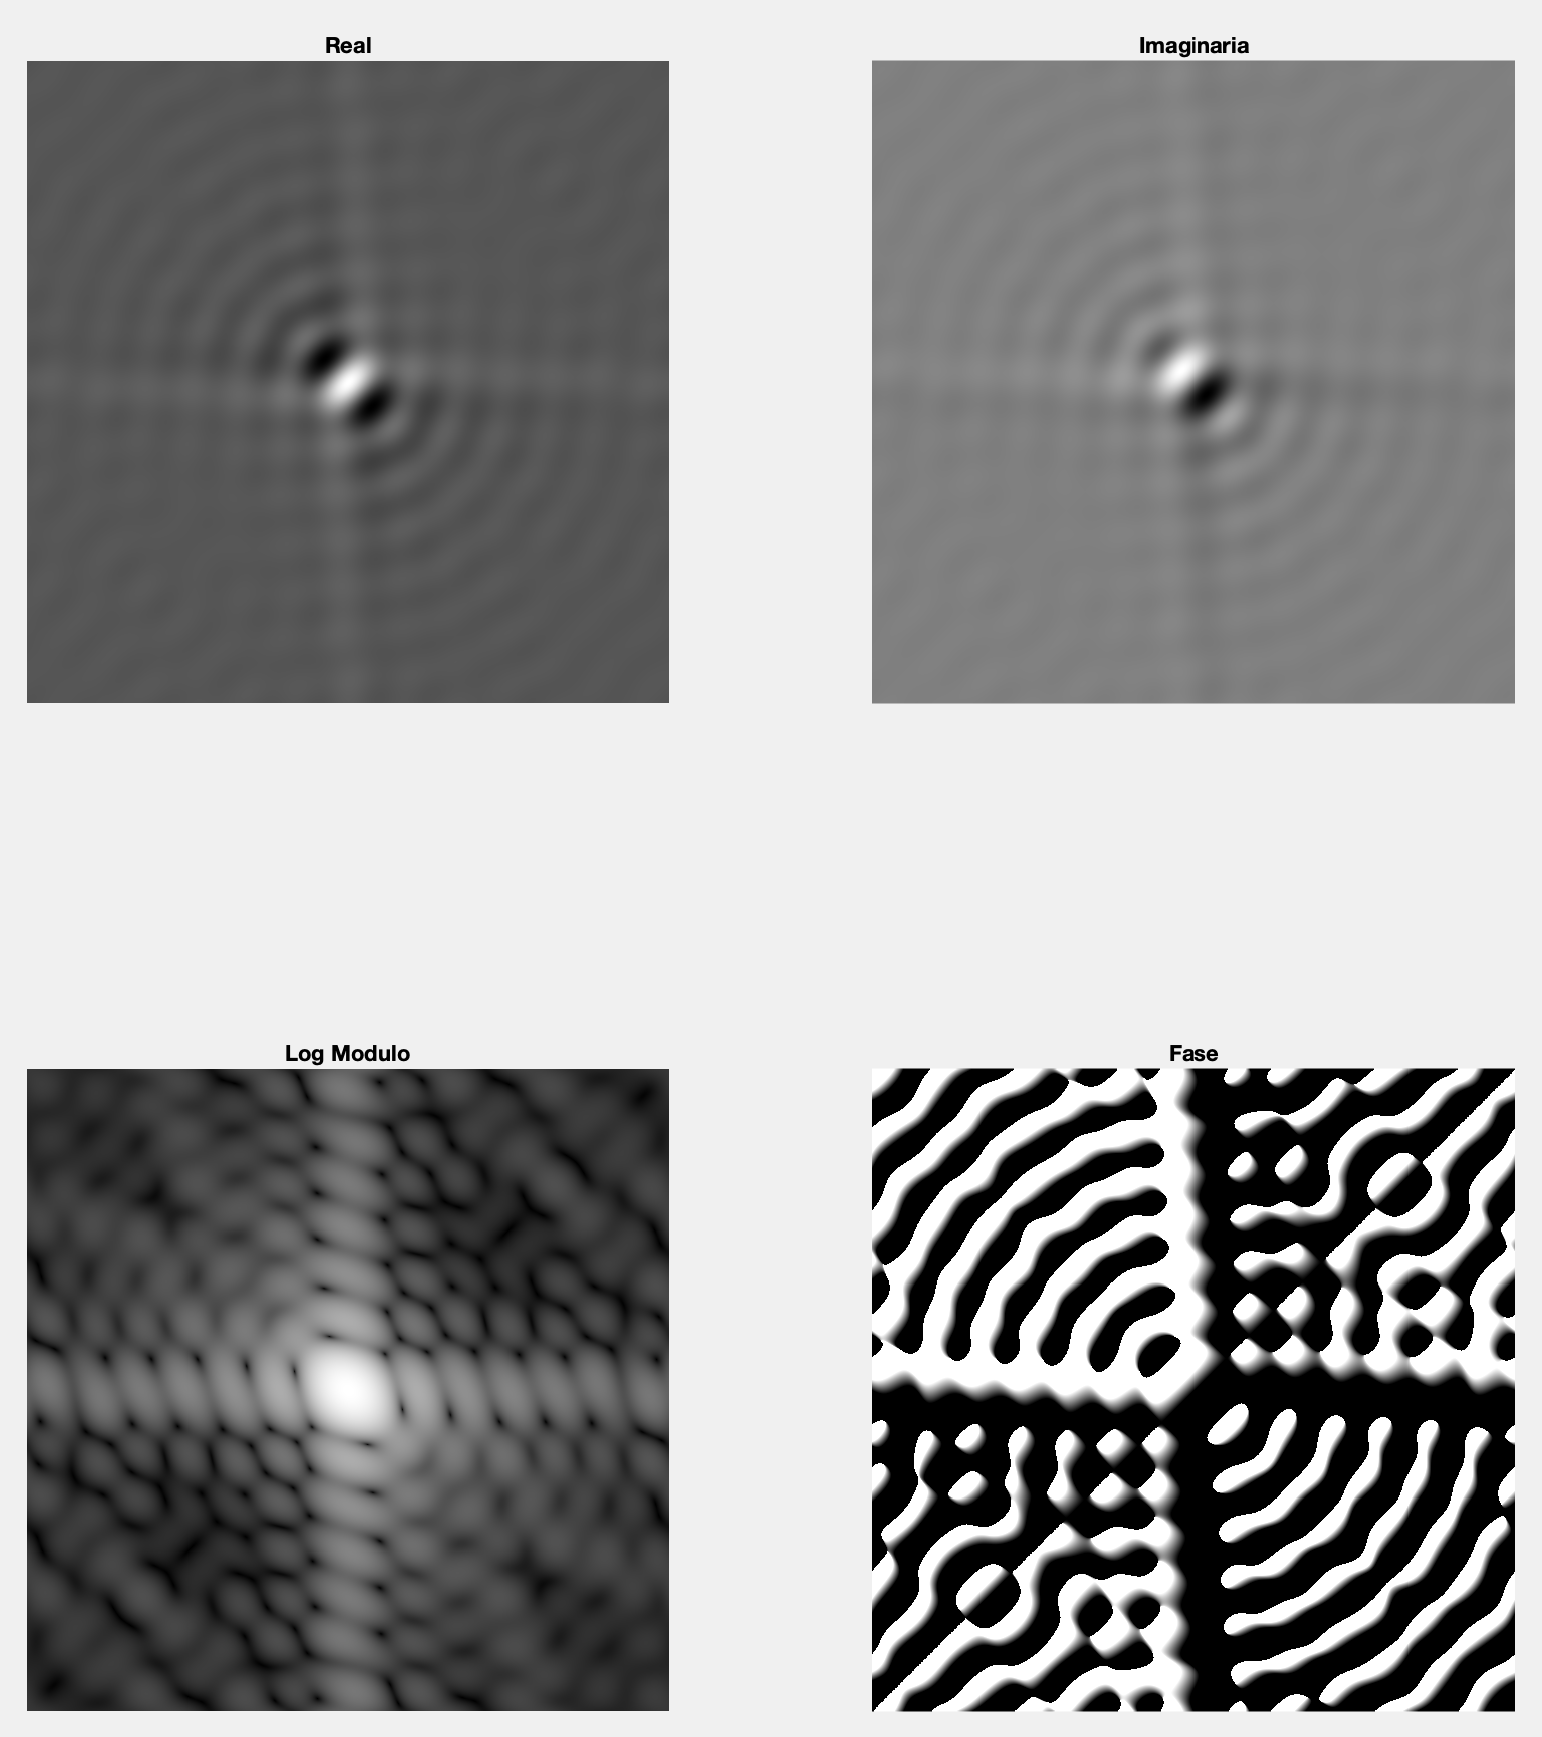
\includegraphics[width=0.3\linewidth]{images/f2.png} & 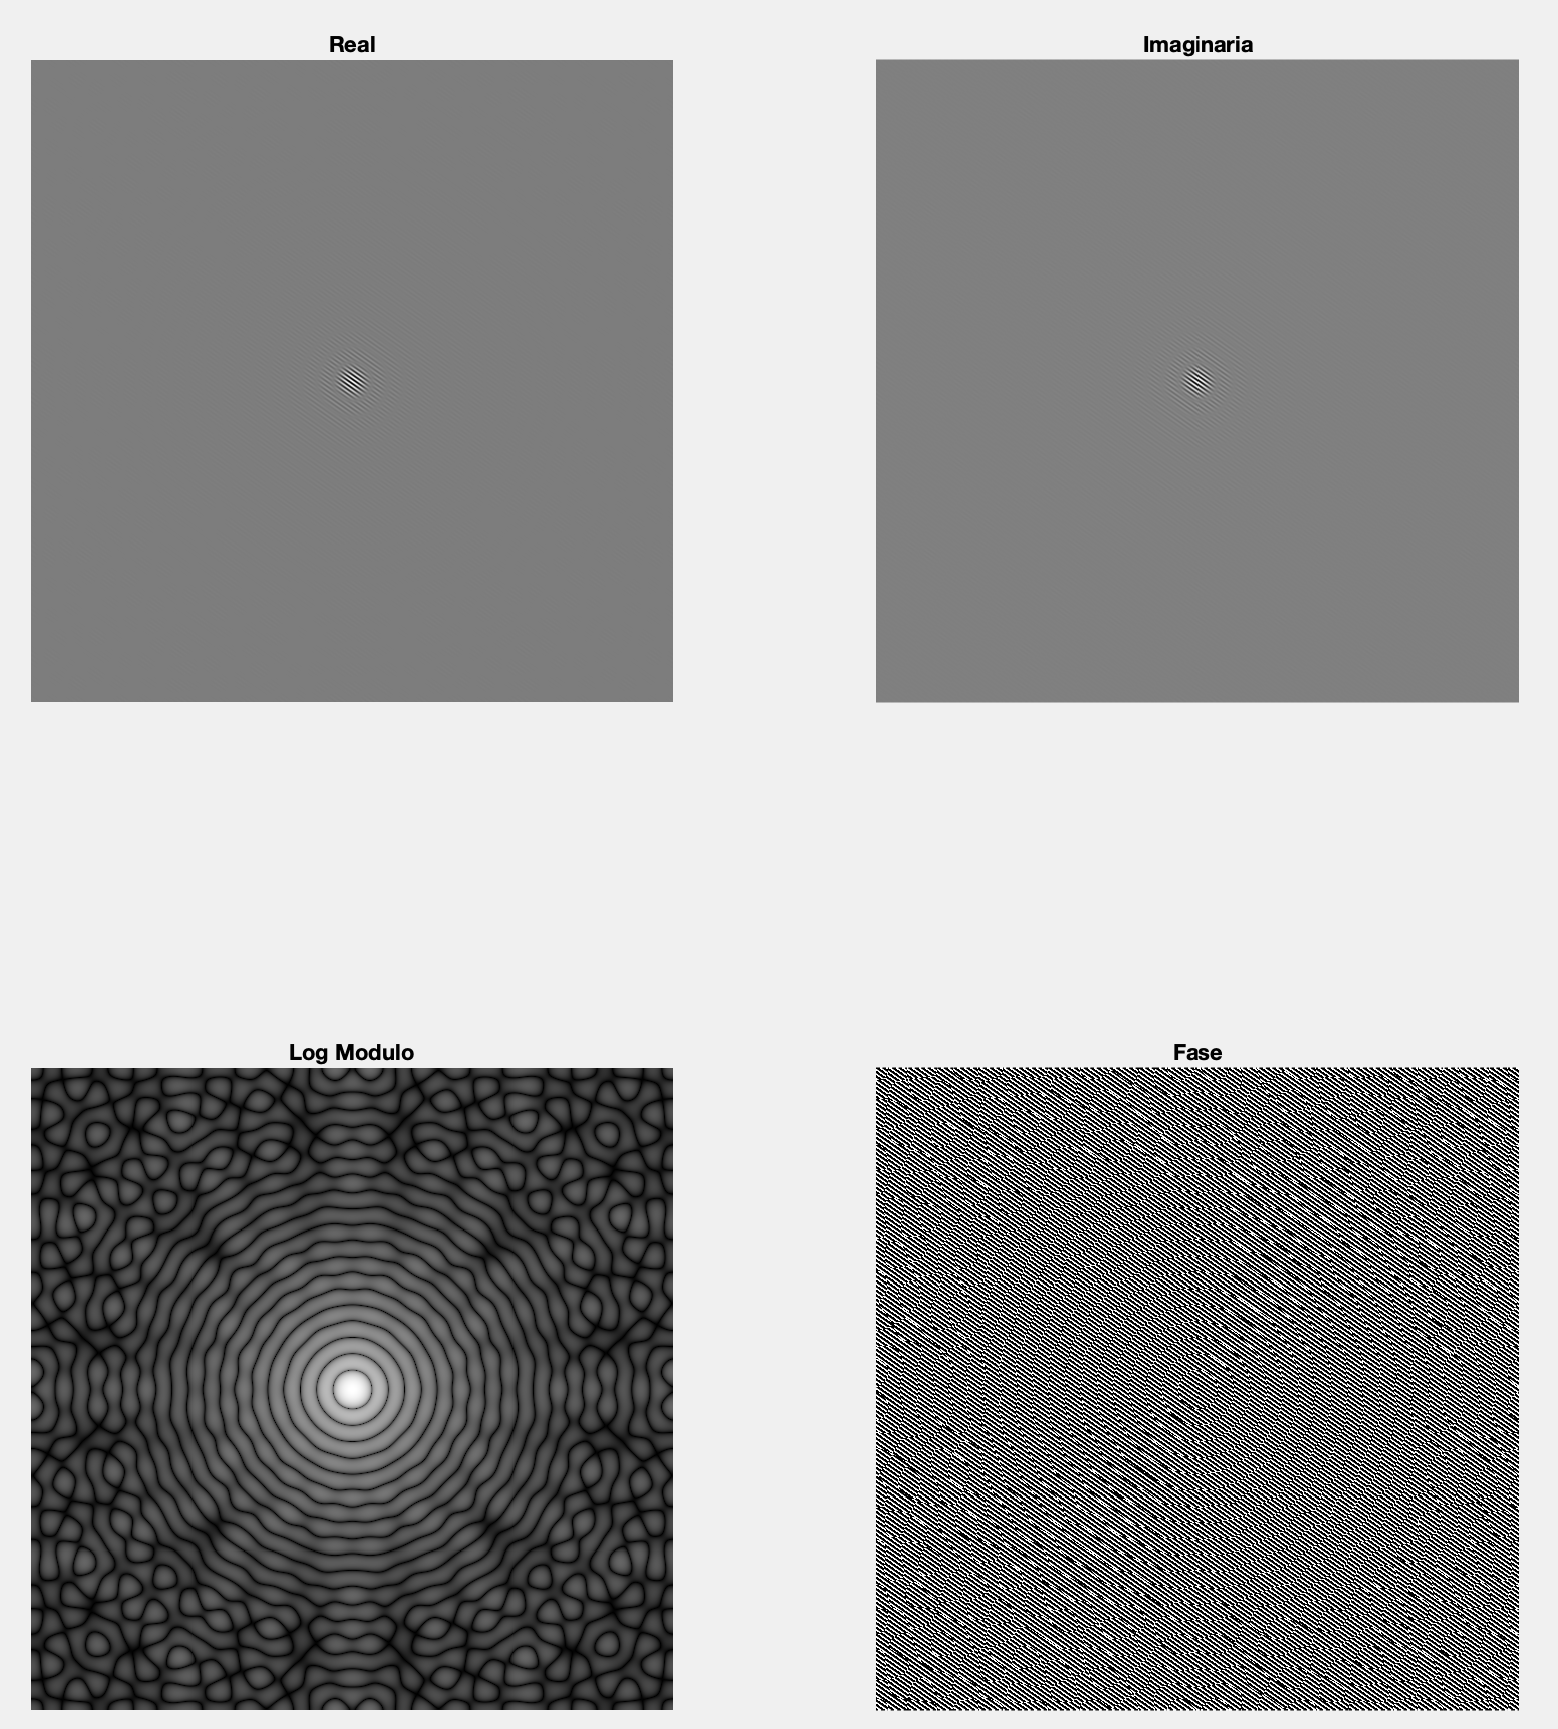
\includegraphics[width=0.3\linewidth]{images/f3.png}
	\end{tabular}
\end{table}

\section{Wavelet.}

A continuación se muestran las reconstrucciones de una imágenes a partir de sus coeficientes \textit{wavelet} cuando cogemos sólo un porcentaje de los mismos:

\begin{figure}[H]
	\centering
	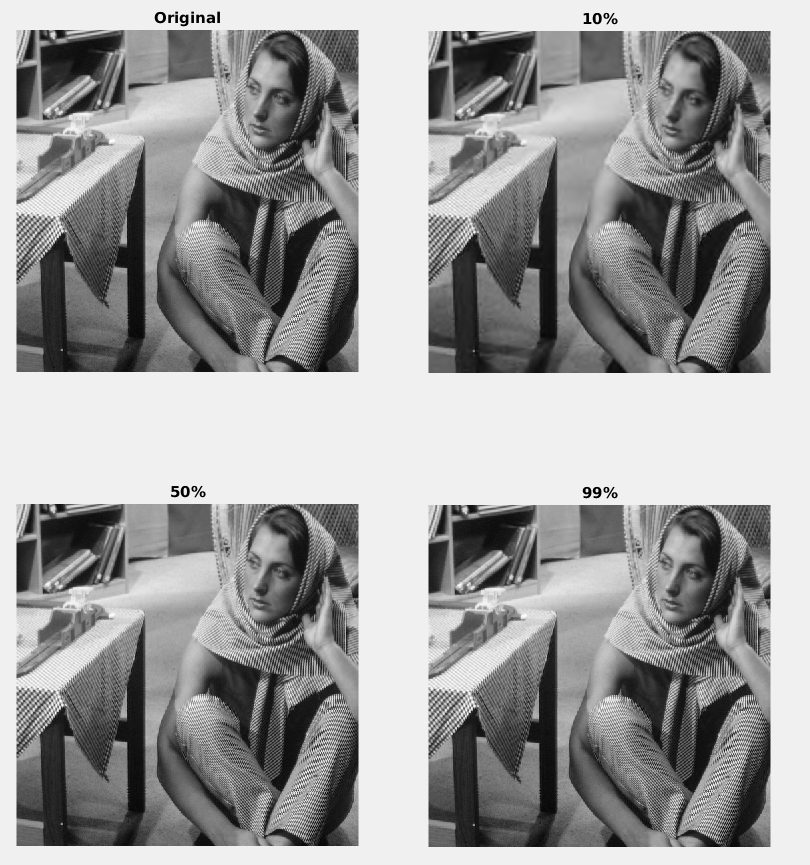
\includegraphics[width=0.8\linewidth]{images/wavelet.png}\\
\end{figure}

Como podemos ver, si nos fiajmos en detalles como los libros o la cara de la mujer, si apreciamos diferencias, pero los resultados son bastante buenos cuando usamos sólo un porcentaje de dichos coeficientes. A continuación se muestra una gráfica con el ratio de compresión en el eje \textit{x} y el valor del \textit{psnr} en el eje \textit{y}:

\begin{figure}[H]
\centering
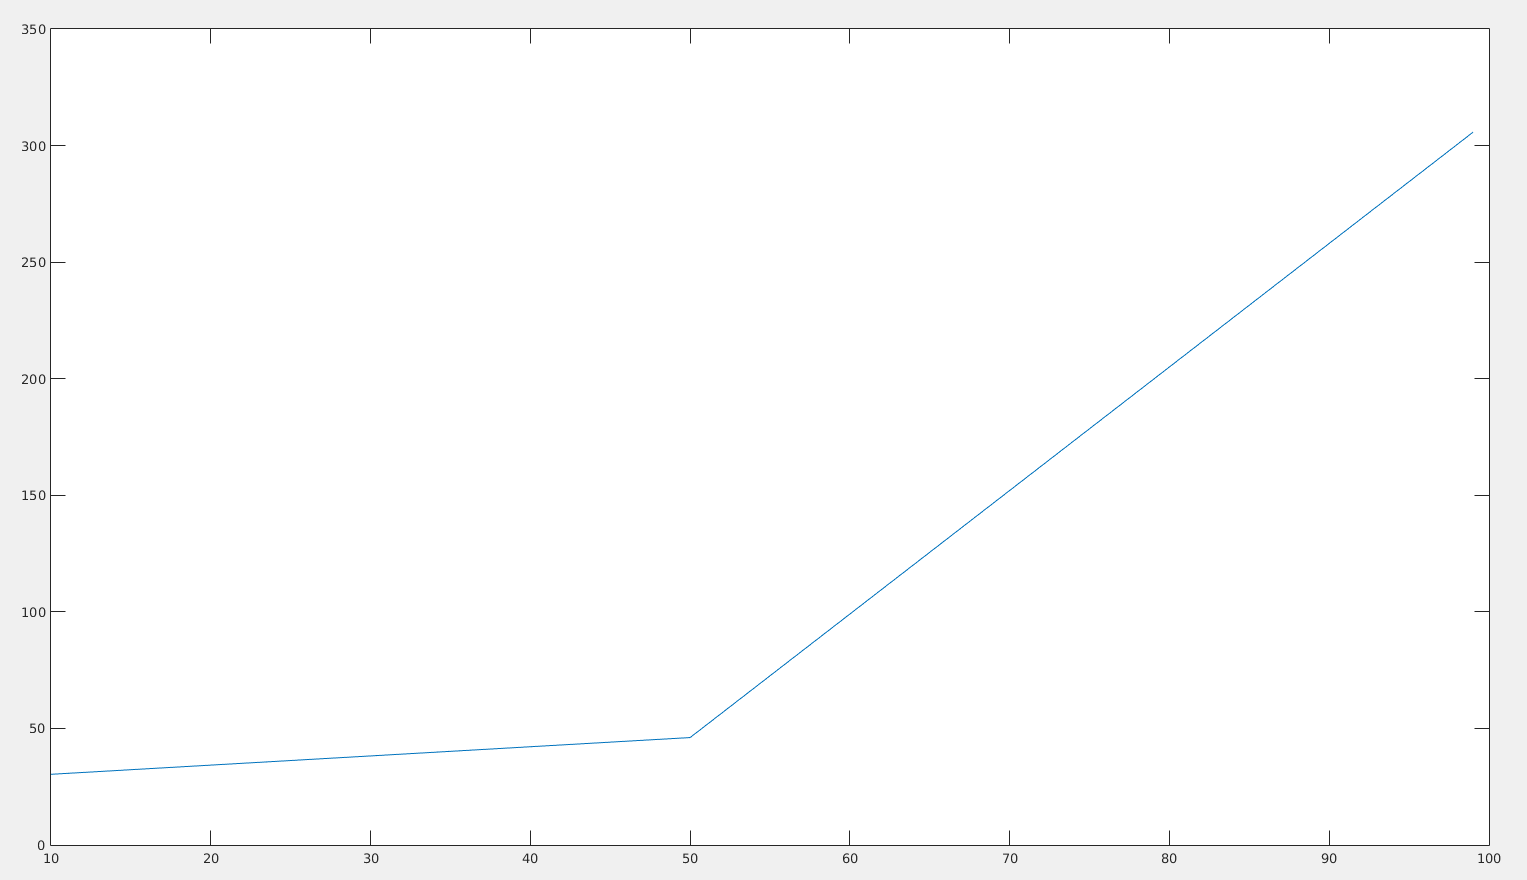
\includegraphics[width=0.8\linewidth]{images/grafica.png}\\
\end{figure}

Cómo podemos ver en el plot, no hay mucha diferencia entre usar el 10\% de los coeficientes o usar el 50\% pero si la hay entre usar el 50\% o usar el 99\%.

\end{document}